\documentclass[a4paper,12pt]{report}
\usepackage[latin1]{inputenc}
\usepackage[english]{babel}
\usepackage{graphicx} 
\usepackage{listings}
\usepackage{fancyvrb}
% \usepackage{bera}% optional: just to have a nice mono-spaced font
\usepackage{xcolor}

\colorlet{punct}{red!60!black}
\definecolor{background}{HTML}{EEEEEE}
\definecolor{delim}{RGB}{20,105,176}
\colorlet{numb}{magenta!60!black}

\lstdefinelanguage{JSON}{
    basicstyle=\normalfont\ttfamily,
    numbers=left,
    numberstyle=\scriptsize,
    stepnumber=1,
    numbersep=8pt,
    showstringspaces=false,
    breaklines=true,
    frame=lines,
    backgroundcolor=\color{background},
    literate=
     *{0}{{{\color{numb}0}}}{1}
      {1}{{{\color{numb}1}}}{1}
      {2}{{{\color{numb}2}}}{1}
      {3}{{{\color{numb}3}}}{1}
      {4}{{{\color{numb}4}}}{1}
      {5}{{{\color{numb}5}}}{1}
      {6}{{{\color{numb}6}}}{1}
      {7}{{{\color{numb}7}}}{1}
      {8}{{{\color{numb}8}}}{1}
      {9}{{{\color{numb}9}}}{1}
      {:}{{{\color{punct}{:}}}}{1}
      {,}{{{\color{punct}{,}}}}{1}
      {\{}{{{\color{delim}{\{}}}}{1}
      {\}}{{{\color{delim}{\}}}}}{1}
      {[}{{{\color{delim}{[}}}}{1}
      {]}{{{\color{delim}{]}}}}{1},
}
\bibliographystyle{unsrt}
\begin{document}

\begin{titlepage}
\begin{center}

\includegraphics[width=5cm]{EURECOM_logo_quadri}
\\[3cm]
\textbf{\Huge{Building ``betterMail''}}
\\[2cm]
\textbf{\textsc{\LARGE{Semester Project Report}}}
\\[0.5cm]
\LARGE{Alessandro Artoni}
\\
\large{Spring 2013}
\\[8cm]
\columnsep3cm
\begin{tabular}{p{8cm} p{8.5cm}}
\small{\textbf{Supervisors:}\newline
Rapha\"el Troncy\newline
Giuseppe Rizzo} 
&
\small{\textbf{EURECOM\newline Multimedia Department}}
\end{tabular}
\end{center}
\end{titlepage}

 \tableofcontents

\chapter{Introduction}
Since its creation in 1993, email did not change much in the way we use it. It's basic idea is simple: a plain exchange of textual (html) messages through  the internet. Thanks to its simplicity on these days most of us receive a huge amount of emails in a single day which makes almost impossible to focus on what's important to us and leave for later what's secondary.

On the other end this huge amount of informations is not exploited as we could: \emph{Entity Recognition}, \emph{Clustering} and \emph{Semantic Web} are only examples of the technologies that can be applied to take advantage of this giant datasets.

Along with extracting informations from data comes the evolution of the web: from a collection of linked documents or \emph{Web Pages} to full fledged \emph{Web Applications}. Thanks to both the evolution of the development environment (HTML5, CSS3, ECMAScript 5) and the rise of mobile devices the web is fastly becoming the universal platform.



\section*{Motivation for the project}

The need for a new approach to electronic mail is getting bigger and bigger along with the amount of messages we receive daily. Moreover we think the potential of building a clustering algorithm based on the entity recognition system provided by the NERD\footnote{Named Entities Recognition and Disambiguation http://nerd.eurecom.fr} framework developed in the Multimedia research group in Eurecom is very high and valuable for improving emails systems.


\chapter{Similar projects}
%Shorten this chapter, and just put short description of the projects, and the conclusions as found in the presentation from week 1 ?

There is a lot of excitement about building and innovating the world of emails, both in universities and in IT companies. We studied some existing projects in order to understand what tecniques were already been used, what are the major approaches used by todays systems and how we can build emails applications better.


These are the projects we study in particular for mining data:
\begin{itemize}
\item Manu Aery and Sharma Chakravarthy developed eMailSift \cite{Aery2005}: an email classification system based on structure and content. They propose a supervised data mining technique based on the exploitation of the structure informations present in email messages.
\item In \cite{Drezde2008} is described an approach to determine if a message should be ``replied to'' or if it ``requires attachments''. Although the focus is very specific it's interesting to see that their approach used a global training set to try to make guess without a specific training set for each user. This idea lend us to think that clustering was to be preferred with respect to classification.
\item The CNR developed a system described in \cite{Manco2008} for \emph{Mining Categories for emails via clustering and pattern discovery}. It's based on a three step approach: k-means for clustering, FP-Growth to extract cluster description and a custom technique to update cluster description.
\end{itemize}

Considering the development of a Web Application as important as the clustering feature, we studied some of the commercial offer (or proposal) available on the market this day:
\begin{itemize}
\item GMail (\texttt{http://mail.google.com}) It's by far the leader in the market and it's considered to be the first \emph{AJAX} web app to be developed. While it offer some ``intelligent'' service (attachment prediction, ``important'' email labeling) it should be credited for building a great UI along with a reliable system.'
\item Alto Mail (\texttt{https://login.altomail.com/login/signin}) while still in closed beta and not available for the public (we didn't manage to try it out) aims to provide better understanding of email subscriptions: they state that Alto Mail understands that products like Facebook, Twitter, LinkedIn, Amazon, (and more?) regularly send notifications and receipts and make it easy to classify or group them. 
\item As a UI starting point we studied MyMail (\texttt{http://dennyshess.ch/mymail/}) which is a mocked up email web client. It's interface allow to manage a lot of differents email folder at the same time, which is why we chose to it.
\end{itemize}
We consider many others papers and articles where, those selected represent the most significant for the development.
 

\chapter{Architectural overview}
In the next chapters we are going to analyze the choice made while designing the system along with some technical description and specification about the implementation. This chapter is divided in three section which reflects the main parts of this project itself: the first part describe the overall architecture of the system, the second section details the implementation of the server-side part of the system together with the specifications of how the clustering algorithm works. In the last part we will describe the prototyping of the client side web application.

Although this document tries to separate as much as possible this three aspect we must point out that both the design and the development of the applications was much more parallel than sequential and so are some technical considerations regarding the overall architecture.

The application \emph(bettermail) is designed with this goal: provide an intelligent system capable of extracting semantic information from the emails body and use them to automatically classify (label) emails. We investigate how a named entities based clustering approach could prove itself in make the email experience better by automating the email labeling process. Moreover the project aims to give the user a simple and intuitive user interface to access those information.

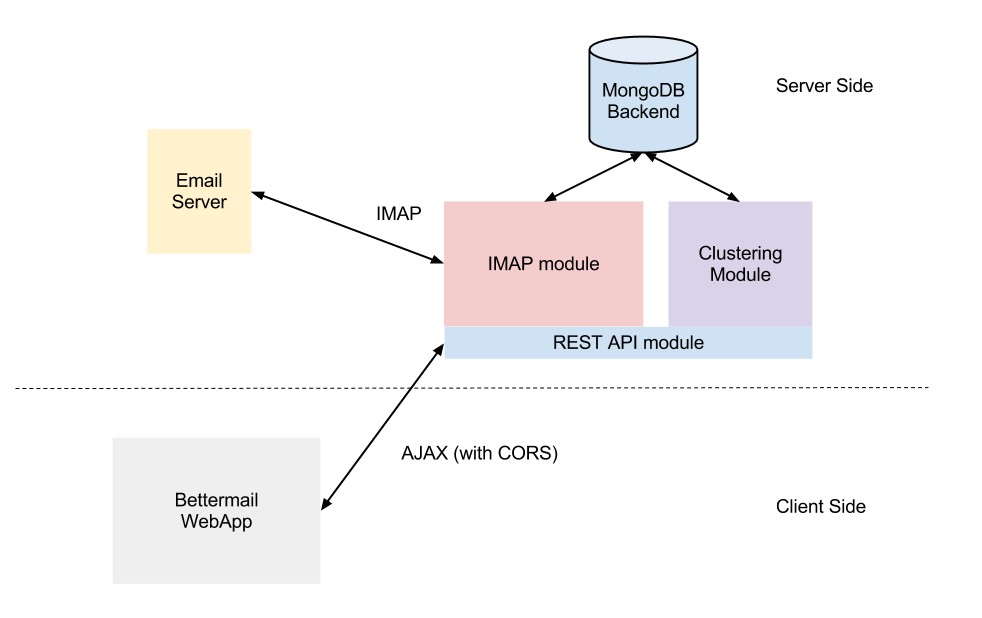
\includegraphics[width=15cm]{Architecture_Overview}
As described in the picture above the application is strongly separated in two parts: client and server side. Because the main idea is to build the client as a SPA\footnote{Single Page Application - http://en.wikipedia.org/wiki/Single-page\_application} and at the same time to make the server functionalities available to potentially more then one client-side application we propose REST\footnote{Representational State Transfer - a style of software architecture for distributed system} as the layer for building the main communication infrastructure. 
We first choose GMail as the targeted email service (mostly because of its wide diffusion) but the final choice is to use a generic IMAP connection to offer better integration with various email provider (although the application is developed and tested with GMail).
\chapter{The Server}

The design and development of the server is one of the major activities of this project. Because our goal is to build a working application prototype from the ground up we first need to get the integration with an existing email provider, thus we build the IMAP module. Next step is to expose this IMAP capabilities and, as discussed previously, we build a RESTfull web service to access it, which allow us to start working on the client too. After that we are finally able to start working on clustering and labeling.

\section{About general technical choices}
The whole server is built using Node.js. It is an event-driven system, built on top of Google's V8 javascript engine which provides a very fast and scalable infrastructure to build server side applications. Because of it's event-driven nature it has proved to be very suitable for I/O intensive application while being comparable to multi-threaded system under a CPU intensive workload. Among performances one of the main idea behind this choice is the developing paradigm. While building an application with a strongly typed language like Java requires a very long and precise designing phase to avoid the need of big refactoring, javascript is generally considered better for fast prototyping and Agile software development \footnote{Although the personal opinion of the author is that javascript can be better even in a more ``classical'' waterfall design end development cycle this matter is too long to be discussed here}.

REST is chosen as the main API access point because of two main reasons: first of all it requires nothing but a client able to use basic HTTP verbs - in contrast with other system like SOAP that requires additional layers or WCF which is specific to a platform - and because it's generally simpler to reason about and define: once the resources' URI are defined the operations on them follows by the definition of RESTfull web service itself. 

All this services relies on a MongoDB powered back-end database which is the natural choice for working in accordance with Agile development and together with Node.js.

\section{Building the IMAP module}
The module responsible for handling the communication with the IMAP server has passed various iterations.
First we tried to build the basic functions to access the IMAP server, query for emails range, add and remove labels and so on\footnote{node-imap (https://github.com/mscdex/node-imap) and mailparser (https://github.com/andris9/mailparser) had been used as a starting point}. 

Subsequently, following the guidelines described in RFC4549\footnote{Synchronization Operations for Disconnected IMAP4 Client (http://www.faqs.org/rfcs/rfc4549.html)} we implemented a basic IMAP client (on the server) with support for incremental syncronization. 
All these feature where then exposed via RESTfull APIs described in the next chapter.

One of the major problems encountered within this phase resides in the sequential nature of the IMAP protocol itself. The first approach was to create a new connection with the IMAP server for each requested resource. While this approach seems fine when tested in a manual request sequence flow it turned out that GMail, like many other providers, impose a very low limit on the maximum number of concurrent request for the same account (it is not specified in the documentation but we experienced it to be around 10). This behavior force us to a fixed, sequential approach, which solved the problem.

\section{The REST server}
For simplifying the process of building our APIs we decided to use the \emph{express} Node.js framework.
Its architecture allow to define ``routes'' on which you can define the behavior for each separate HTTP verb. In addition it provides a system for plug middleware in the system before routes are handled (for example authenticating user before serving the request). We used this feature to implement a CORS\footnote{Cross-origin resource sharing, a new standard to allow web applications to safely bypass the same origin policy} compliant web service.

These are the main resources defined with the associated URI.Except for labels, the service support the GET verb only because the first goal of the application is email reading and retrieving. Anyway the architecture would allow to easily add feature like deleting or sending new emails provided to use an SMTP module which at the moment we didn't yet wrote.
Each method exchanges informations in the JSON format. The structure of the returned item is listed after each resource.
\begin{itemize}
\item \texttt{/boxes}: The list of all the mailbox available.
\begin{lstlisting}[language=JSON]
[
  {
    "attribs": [
      "HASNOCHILDREN"
    ],
    "delimiter": "/",
    "name": "SomeLabelName"
  },
  //...
]
\end{lstlisting}
\item \texttt{/boxes/:boxId}: The details of the mailbox specified by the boxId
\begin{lstlisting}[language=JSON]
{
  "uidnext": 293,
  "readOnly": true,
  "flags": [
    "Answered",
    "Flagged",
    "Draft",
    //...
  ],
  "newKeywords": false,
  "uidvalidity": 30,
  "keywords": [
    ""
  ],
  "permFlags": [],
  "name": "SomeLabelName",
  "messages": {
    "total": 279,
    "new": 0
  }
}
\end{lstlisting}
\item \texttt{/boxes/:boxId/:mailUid}: The full body of the specified email (identified by \texttt{boxId} AND \texttt{mailUid})
\begin{lstlisting}[language=JSON]
{
  "text": "someText",
  "html": "<html>someHtml</html>",
  "headers": {
    "delivered-to": "artoale@gmail.com",
    "received": [...]
    //...
  },
  "subject": "aSubject",
  "references": [
    // Related email messageId
  ],
  "messageId": "aMessageId",
  "inReplyTo": [
    "anotherMsgId"
  ],
  "priority": "normal",
  "from": [
    {
      "address": "someOne@gmail.com",
      "name": "Some One"
    }
  ],
  "to": [
    {
      "address": "me@gmail.com",
      "name": "Alessandro Artoni"
    }
  ],
  "seqno": 146,
  "uid": 153,
  "flags": [
    "\\Seen"
  ],
  "date": "24-Oct-2010 18:10:53 +0000",
  "_events": {},
  "x-gm-thrid": "1350194035284457856",
  "x-gm-msgid": "1350507014051968106",
  "x-gm-labels": [
    "\\\\Inbox",
    "\\\\Important"
  ]
}
\end{lstlisting}
\item \texttt{/boxes/:boxId/unseen}: The headers and mime structure of  all the unseen emails in the specified mailbox
\begin{lstlisting}[language=JSON]
[
  {
    //an object like the previous example but without text and html 
  },
  //more objects...
]
\end{lstlisting}
\item \texttt{/boxes/:boxId/:mailUid/labels}: The list of labels assigned to the specified email
\begin{lstlisting}[language=JSON]
[
  "\\\\Inbox",
  "\\\\Important",
  //...
]
\end{lstlisting}
\item \texttt{/boxes/:boxId/from/:startUid}: The structure and headers of all emails in a specific mailbox with an UID strictly bigger than \texttt{startUid}.
\item \texttt{/boxes/:boxId/from/:startUid/to/:endUid}: The structure and headers of all emails in a specific mailbox with an UID ranging from \texttt{startUid} (excluded) to \texttt{endUid}(included). If \texttt{endUid} is bigger then the maximum UID available this URI is equivalent to the previous one.
\item \texttt{/sync/:boxId}: Start a new synchronization of the specified mailbox. This URI fires the synchronization mechanism described in the previous section.
\end{itemize}

\section{Named Entity Recognition}
Each email content is first parsed by the NERD framework thanks to the node module provided by the team\footnote{https://github.com/giusepperizzo/nerd4node}. The email body is then annotated with a set of informations; for our work we considered two of them: \texttt{NerdType} which represent the ``high level'' class of the part of the text considered (e.g. Person, Thing, Date ...) and \texttt{label}, the specific entity recognized by NERD (e.g. Barack Obama, Personal Computer, 2012 ...). 
Those informations are then stored permanently on the database for subsequent elaboration.

\section{The clustering algorithm}
The basic idea behind the approach to labeling emails is divided in three step: named entity recognition, starting centroids definition and clustering. This technique is inspired by that described by \cite{Manco2008} but it tries to exploit as much as possible the structured informations from the email.



\subsection{Defining Centroids}
Instead of using a pure k-means approach with random starting centroids we choose to firt use an Agglomerative Hybrid Clustering (AHC) implementation on a randomly selected subsets of emails. This algorithm outputs a three known as a \emph{dendogram} in which each node correspond to a partition of the clusters and it's child as progressive sub-partitions. We traverse this three selecting all the node smaller then a parameter $L$ as basic clusters.
For each of this base clusters (if they're bigger than $L/k$ with $k$ parameter) we pick a random element in it as one of the starting centroids for the next step.

\subsection{K-Means}
The last step in the clustering algorithm is to apply a slightly modified version of k-means with \emph{linkage} criterion. As described above: instead of starting from randomly selected centroids we tried to exploit some knowledge to improve the clusters quality. While the AHC was executed on a subset of emails for performances reason, we run k-means over the whole dataset.

\subsection{Metrics}
We gradually added features ($F_{i}$) to the definitions of our distances functions (one for each algorithm):
\begin{itemize}
\item $F_{1}$: NERD type extracted (only if text field available, no HTML)
\item $F_{2}$: Email address (in both \emph{from} and \emph{to} fields)
\item $F_{3}$: Datetime 
\item $F_{4}$: Named entity label
\end{itemize}

This features are then used to computed a coefficient $C_{i}$, one per feature, with this relationship:
\[C_{i} = F_{i}^3 / 3 \]
Each coefficient is then normalized and multiplied by a wheight $w_{i}$, depending on the clustering technique used as follow:
\[distance = 1 - \sum_{i=1}^{4} g(C_i)*w_i \]
where $g$ is a function for normalizing values between 0 and 1 and $w$ is $[0.7, 0, 0, 0.3]$ for AHC and $[0.4, 0, 0.1, 0.5]$ for k-means.
\chapter{Building the client}
Multiple approaches on which type of client to develop are available. Among other ideas the two main possible approaches we consider are:
\begin{itemize}
\item adding feature to an existing web client (GMail, Hotmail, etc...) by using either public APIs provided or by hacking the basic website by introducing script with browser extensions (Greasemonkey, Tampermonkey, ...)
\item creating a basic email web client from scratch
\end{itemize}

Because the first approach seems more reasonable in terms of time and efforts we pick it as first choice, specifically targeting GMail. After few tries with prototyping and reading a lot of documentation\footnote{https://developers.google.com/gadgets/} two problems arise: first of all the main APIs for adding functionalities to gmail is deprecated and won't be supported after July 2013. On the other end as the term itself suggests, hacking the website is full of problems: programming it's tedious, it requires a lot of DOM manipulation and traversing, done without a clear specification of how the HTML is structured and thus, how to manipulate it and there is no guarantee for the page structure not to change without notice.

For this reason our final solution is a basic, web based, email client.

\section{Architecture}
As previously noted we decided to implement the client as a SPA. That is because interaction obtained thanks to the intensive use of XHR\footnote{the main object used for sending asynchronous HTTP requests} it's widely considered ways better with respect to the classical multi-page model. In fact most web applications\footnote{the terms doesn't refer to general web sites but to complete applications built on top of the web platform like gmail, Cloud9IDE, google drive...} today prefer this model to offer a faster and more engaging UI to its users. 

To better structure our work we use an MVC javascript framework chosen between Backbone.js, Ember and AngularJS. The first is the oldest and has many interesting feature, but it force users to a specif type of data access, which is pretty far from plain javascript, and doesn't provide by itself a clear, structured way of developing the application. While Ember may be a good choice we choose the latter among those.
Because the choice of a framework strongly effects the overall architecture of the system, on the next session we will explain why we use AngularJS and how this choice effects the client structure.
\subsection{About AngularJS}
The reason behind our choice is to be found in the three main features of this framework, often denoted as \emph{3D} (Data Binding, Directives and Dependency Injection).
\subsubsection{Two ways data binding}
Most client-side frameworks offer some kind of templating system which allow to define how objects will be represented when attached to the DOM. These libraries offer a one-way data binding: if the object changes, the framework is notified and the DOM is altered accordingly.
AngularJS on the other end improve this approach in two ways: it uses plain HTML (even W3C compliant, if required) as the templating system and offer data binding in both directions: not only objects changes are reflected in the DOM, but the other way round too. If an input box is binded with a javascript variable, each time the input box is changed the variable itself is modified accordingly.
\subsubsection{Directives}
Front-end developer usually create or use widget to encapsulate specific behavior in a single piece of code. Thanks to \emph{directives} it is possible to extend the native HTML markup language by \begin{quotation}
``teaching the browser new tricks''.
\begin{flushright}
Pavel Kozlowsky, Codemotion, Rome - 23 March 2013\footnote{http://www.youtube.com/watch?v=wmhPfx0s40o}
\end{flushright}
\end{quotation}
In other words it is possible to define your own tag and then use them like they were plain HTML; AngularJS compile them in an internal representation and attach the real HTML on the fly.
This feature provides two big advantages: you can build highly reusable components and the code looks much more cleaner and readable thanks to the markup being embedded in the directives. 
\subsubsection{Dependency Injection}
One of the main feature required by a industrial-ready system is to provide an easy way to unit test your components. AngularJS encourage developers to write separate modules; each module specify the list of other modules it depends on, without explicitly allocating the resource (process handled by the framework). ``requiring'' something instead of directly ``creating'' it make the components of an application much more decoupled (and thus, easier to maintain). Moreover thanks to the ability to use different implementation of a specific component depending on the environment it become much easier to test this component independently: it is sufficient to provide a ``mocked'' version of a dependencies to avoid the need of having an instance of the real dependency up and running (this can be very useful if the dependency rely on some external service, it's slow or requires the system to change state, which is bad for unit testing).


As AngularJS is our framework of choice, the application follow the structure described by the framework itself:
\begin{itemize}
\item a set of \emph{service}s is responsible for creating an abstraction layer to access data. In our case we have services for retrieving data in the IndexedDB storage system of the browser (described later) and a service for accessing the REST API of our server.
\item a set of \emph{directive}s to encapsulate the behavior behind the graphical components of our applications 
\item some \emph{controller}s, responsible for binding data to the right HTML fragment (including event handlers).
\end{itemize}
\subsection{Tooling, scaffolding and external libraries}
In the last few years a lot of efforts have been put in improving and automating the workflow of front-end web development. A lot of tools and systems have been created in order to reduce developers efforts. 
Moreover, together with AngularJS we used other external resources to speed up and simplify the process. Here's a list of tools and external libraries of invaluable worth:
\begin{itemize}
\item Yeoman (yo - \texttt{http://yeoman.io}): a tool for project scaffolding. It creates a template web application including HTML5 boilerplate, EscmaScript 5 polyfill and many optionals libraries. Thanks to its excellent integration with AngularJS it can be invoked each time we need to create a new angular component (e.g to create a directive called tab \texttt{yo angular:directive tab}). Moreover it creates a complete and customized configuration file for \emph{Grunt}, described below
\item Grunt (\texttt{http://gruntjs.com}): used to build, preview and test the project, thanks to the help from tasks created using Yeoman it's very well integrated in the ecosystem. Specifically, it allows to run a static web server to serve file and try the systems, automatically compiles coffescript into javascript and SASS/SCSS into plain CSS every time a file changes, add support for in-browser livereload (again, on file changes). It integrates with Karma-runner, the javascript test runner developed by the AngularJS team. It allows to build the application by minifying and eventually optimizing javascript and CSS, compressing images and much more.
\item Bower (\texttt{http://bower.io}): it offers a solution to the front-end package management problem, as it allows to maintain and manage package installations and dependencies for generic front-end development resources (typically javascript and CSS libraries). 
\item Twitter Bootstrap (\texttt{http://twitter.github.io/bootstrap/}): a stylesheet framework which simplifies the development of user interfaces. It provides a grid system for layout definition and a wide set of components (buttons, tables, tooltips, etc...) 
\end{itemize}
\section{Design}
Lorem ipsum dolor sit amet, consectetur adipisicing elit. Sequi, distinctio, voluptatum ratione recusandae perferendis laboriosam illum earum dicta consequatur nam.
\subsection{Sketches}
Lorem ipsum dolor sit amet, consectetur adipisicing elit. Amet, pariatur, assumenda, labore ullam libero atque doloribus asperiores quasi est incidunt officia numquam doloremque ut temporibus quis nisi totam cum laudantium tenetur nihil et! Saepe, impedit maxime commodi ab minus provident sunt cupiditate voluptates veritatis eveniet ex expedita dolorum dolorem non minima perspiciatis beatae porro soluta officiis nihil eligendi aliquid explicabo eum. Deserunt, commodi voluptatem eligendi nobis nihil libero ducimus sunt distinctio asperiores ratione porro quam quae vel modi sit necessitatibus explicabo magnam ipsa ad suscipit blanditiis cupiditate ipsam error illum voluptates dicta cum consectetur quibusdam eius quas beatae reiciendis laudantium possimus. Officiis, ab voluptatibus corporis quam assumenda harum facilis illo ex dolorem sunt doloremque hic unde repellat facere dolores accusantium soluta! Architecto, magnam nobis maiores beatae fuga sed voluptatibus cum nisi reiciendis iure id eum rem nihil velit non veritatis aliquam. Officiis, incidunt, itaque, perspiciatis reiciendis at ex consequatur tempora vel dolor commodi beatae molestias labore aut porro numquam architecto illum quae maiores blanditiis eaque quis reprehenderit enim amet cumque adipisci? Reprehenderit, animi, qui, quia repudiandae nam esse pariatur facere blanditiis aperiam inventore consequuntur voluptates dignissimos provident vel praesentium! Vero, nihil, consectetur magni possimus ratione ullam neque totam accusantium porro.
\subsection{Prototypes}
Lorem ipsum dolor sit amet, consectetur adipisicing elit. Tempore, sapiente, odio, provident animi veniam incidunt vel blanditiis atque voluptatem laborum eveniet eligendi dignissimos libero amet natus ullam odit sint voluptatum saepe officiis iusto obcaecati itaque illo praesentium porro iste nulla quibusdam commodi aliquam. Qui, doloribus, quasi, alias cum neque nisi laborum quis porro hic quaerat inventore blanditiis voluptas nihil unde rerum repellendus quae. Molestias, numquam, expedita odio adipisci tenetur quasi animi sint veritatis placeat voluptatum dignissimos earum impedit maxime nulla accusamus doloribus atque magnam provident consequuntur quia quibusdam hic obcaecati inventore et ipsum quo similique odit itaque aperiam assumenda laborum sed dolorem quidem vitae corporis excepturi fugit! Illum, vel numquam esse corrupti facilis eaque mollitia praesentium harum assumenda a doloribus et eveniet iste asperiores optio doloremque ratione explicabo ut natus necessitatibus voluptate corporis sit vero sint saepe quos aliquam nobis cumque aspernatur non repellendus perspiciatis eum quas. Quo, iure, suscipit, aspernatur ipsum dignissimos assumenda enim aliquid velit impedit voluptatum omnis eligendi cumque incidunt quaerat quidem maiores inventore ratione officia facilis fuga dolorem quia voluptate quam consequuntur animi repudiandae natus nostrum! Modi, perspiciatis, eveniet, nostrum dolores ab fugit eum tempora eos iusto vel illum pariatur quibusdam temporibus officia quam enim necessitatibus ut eius libero nulla repellat. Quaerat, aut, voluptates, hic, commodi officia rerum nam consectetur necessitatibus fugiat ea vero atque voluptatem harum magnam expedita quam magni ab incidunt. At, magnam, fuga corporis rem vitae laborum veniam quos error aut minima ea odit itaque explicabo ducimus harum sint impedit neque recusandae ratione dignissimos quam maiores nulla natus sequi molestias libero necessitatibus amet perferendis pariatur eos saepe qui odio deleniti nemo commodi dolores ipsam consequuntur in autem magni. Saepe, quisquam ex odio dicta optio aut provident autem reprehenderit veritatis expedita illo eveniet ab rerum quas facilis aliquam quo corporis vero laudantium eos dolore!
\subsection{Final result}
Lorem ipsum dolor sit amet, consectetur adipisicing elit. Voluptate, amet repudiandae eaque saepe molestias inventore perspiciatis iste natus doloremque quo soluta temporibus ea minima veniam ipsam incidunt rem ut non accusantium corrupti veritatis autem a culpa suscipit laborum? Quam in tempora at sequi nobis eaque culpa. Ab, cupiditate, distinctio, rem, fugit sunt porro quae optio eveniet molestias reiciendis deleniti dolorum. Repudiandae, praesentium, placeat, ab, ipsum culpa sed illum sapiente quis eaque porro dolore facere quae nam ullam beatae laborum impedit amet officia asperiores accusantium laboriosam non deserunt aspernatur voluptate enim accusamus doloremque. Eaque quod officiis sed unde dolores repellendus quae!
\chapter{Evaluation}
\section{Analysis on a personal dataset}
\section{Metric measures on ``enron'' dataset}
\chapter{Conclusion/Future work}
Lorem ipsum dolor sit amet, consectetur adipisicing elit. Quas, debitis accusantium ratione maxime veritatis eveniet nisi laborum cum labore libero modi amet odio inventore ipsum facere non voluptatum velit natus hic beatae quaerat fuga accusamus fugit excepturi perspiciatis aperiam neque aut culpa autem porro ea minus repudiandae aspernatur quam ducimus molestias eaque. Praesentium, odit, est, eos distinctio debitis repudiandae vero deleniti nihil molestiae sit ab reprehenderit tempore! Quibusdam, saepe, minima, libero, iure temporibus voluptate doloremque aliquid maxime nam deserunt quam odit illo voluptatibus ducimus non recusandae nesciunt ratione dicta consequuntur cumque. Esse, molestias, inventore labore incidunt quas distinctio perferendis animi odio ab ratione cupiditate qui eum aliquam? Deleniti, delectus nesciunt at quas eligendi fuga provident mollitia perferendis magnam laboriosam officia eaque harum animi culpa reprehenderit voluptate repellat iure quasi temporibus autem illo nemo sed quo eveniet laborum a similique nostrum rem adipisci rerum sint voluptatum accusantium ea. Asperiores, incidunt, non atque cupiditate fuga quasi perspiciatis. Deserunt, debitis nemo laudantium vero nisi qui enim voluptatum minus animi asperiores eius maiores voluptates atque voluptate dolores. Porro, voluptas, minus, rem asperiores fugiat eligendi commodi hic debitis eaque voluptates optio esse laudantium odit ab sequi harum recusandae amet iusto tempora expedita nisi reiciendis accusantium quisquam veritatis ipsam. Placeat, magni, rerum ipsam est a explicabo cupiditate repudiandae odit praesentium temporibus sequi voluptatem harum officia consequuntur laborum necessitatibus facilis! Numquam, expedita, iusto, animi laborum nihil omnis culpa impedit quisquam tempora adipisci iste odio nisi ducimus assumenda sint aut molestias. Cumque, doloremque, nemo, magni pariatur maxime adipisci nihil quibusdam ipsa earum perferendis alias libero eligendi excepturi voluptatum voluptate quas ullam consequatur voluptates distinctio tempora explicabo consequuntur id nostrum ad numquam maiores architecto fugiat repellendus quod beatae incidunt blanditiis necessitatibus aut quisquam quasi rem culpa. Id, maxime, autem, perspiciatis debitis fugit vero quia modi voluptatem temporibus vel similique.
\addcontentsline{toc}{chapter}{Bibliography}
\bibliography{biblio}

\appendix
\cleardoublepage
%\chapter{REVE ontology}
%\includegraphics[page=2,angle=-90, width=1.2\textwidth]{graphs.pdf}
%\chapter{Data model: focus on a person}
%\chapter{Data model: focus on a document}
%\chapter{Present state of the data}
%TODO : arranger l'orientation des pages pr l'impression ?

%\includepdf[pages=1-20]{fichier.pdf}
\end{document}
